\documentclass[a4paper,12pt]{article}

\usepackage[english]{babel}
\usepackage[T1]{fontenc}
\usepackage[utf8]{inputenc}
\usepackage{amsmath}
\usepackage{amsthm}
\usepackage{forest}
\usepackage{graphicx}
\graphicspath{{images/}}
\usepackage{tikz}
\usepackage{tikz-qtree}
\usepackage{graphicx}
\usepackage{xcolor}
\usepackage[colorinlistoftodos]{todonotes}
\usepackage{enumitem}
\usepackage{DejaVuSansMono}
\usepackage{listings}
\lstset{basicstyle=\footnotesize\ttfamily,breaklines=true}
\lstset{frame=tb,language=python,numbers=left,showstringspaces=false}
\renewcommand{\lstlistingname}{Code Block}

\usepackage{geometry}
\geometry{total={210mm,297mm},
left=20mm, right=20mm,
bindingoffset=0mm,
top=20mm, bottom=20mm}

\usepackage[
  pdftitle={Assignment 3},
  pdfauthor={William Jagels},
  colorlinks=true,linkcolor=blue,urlcolor=blue,citecolor=blue,bookmarks=true,
bookmarksopenlevel=2]{hyperref}

\usepackage{titlesec}
\titlelabel{\thetitle.\quad}

\def\code#1{\texttt{#1}}

\title{Assignment 3}

\author{William Jagels}

\date{\today}

\begin{document}
\maketitle

\section{Heap Operations}
\subsection{deleteMin()}
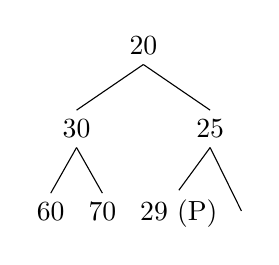
\begin{tikzpicture}
  \Tree [.20 [.30 60 70 ] [.25 {29 (P)} {} ] ]
\end{tikzpicture}

\subsection{insert(5)}
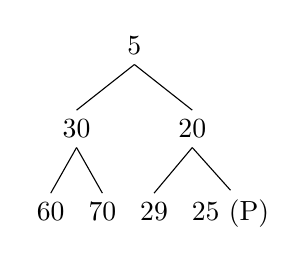
\begin{tikzpicture}
  \Tree [.5 [.30 60 70 ] [.20 29 {25 (P)} ] ]
\end{tikzpicture}

\section{Binary Tree}
\subsection{Essential complete binary tree}
[10 11 7 15 9 3 12 10 22 8]

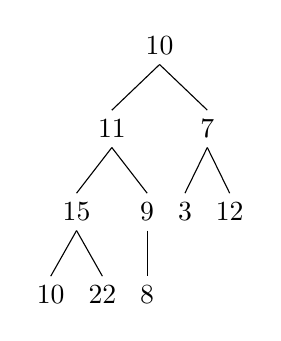
\begin{tikzpicture}
  \Tree [.10 [.11 [.15 10 22 ] [.9 8 ] ] [.7 3 12 ] ]
\end{tikzpicture}

\subsection{Min heap}
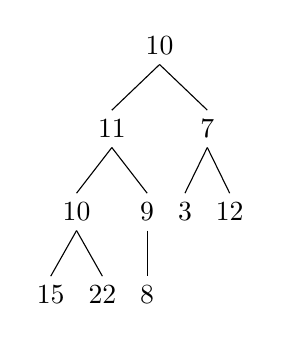
\begin{tikzpicture}
  \Tree [.10 [.11 [.10 15 22 ] [.9 8 ] ] [.7 3 12 ] ]
\end{tikzpicture}

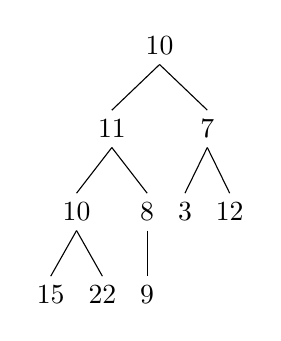
\begin{tikzpicture}
  \Tree [.10 [.11 [.10 15 22 ] [.8 9 ] ] [.7 3 12 ] ]
\end{tikzpicture}

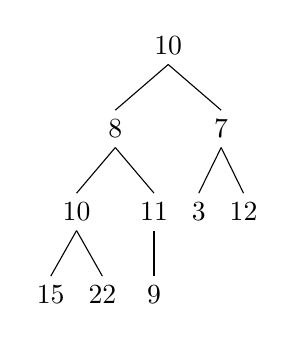
\begin{tikzpicture}
  \Tree [.10 [.8 [.10 15 22 ] [.11 9 ] ] [.7 3 12 ] ]
\end{tikzpicture}

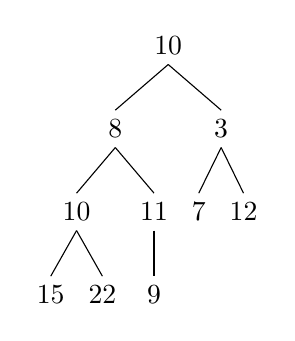
\begin{tikzpicture}
  \Tree [.10 [.8 [.10 15 22 ] [.11 9 ] ] [.3 7 12 ] ]
\end{tikzpicture}

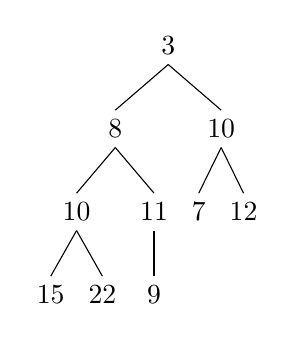
\begin{tikzpicture}
  \Tree [.3 [.8 [.10 15 22 ] [.11 9 ] ] [.10 7 12 ] ]
\end{tikzpicture}

\subsection{Max Heap}
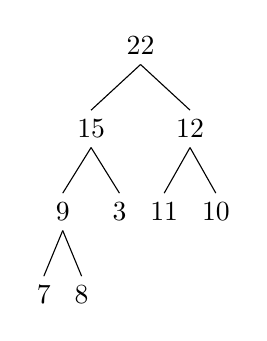
\begin{tikzpicture}
  \Tree [.22 [.15 [.9 7 8 ] 3 ] [.12 11 10 ] ]
\end{tikzpicture}

Sorted: [22 15 12 11 10 9 8 7 3]

\section{LCS}
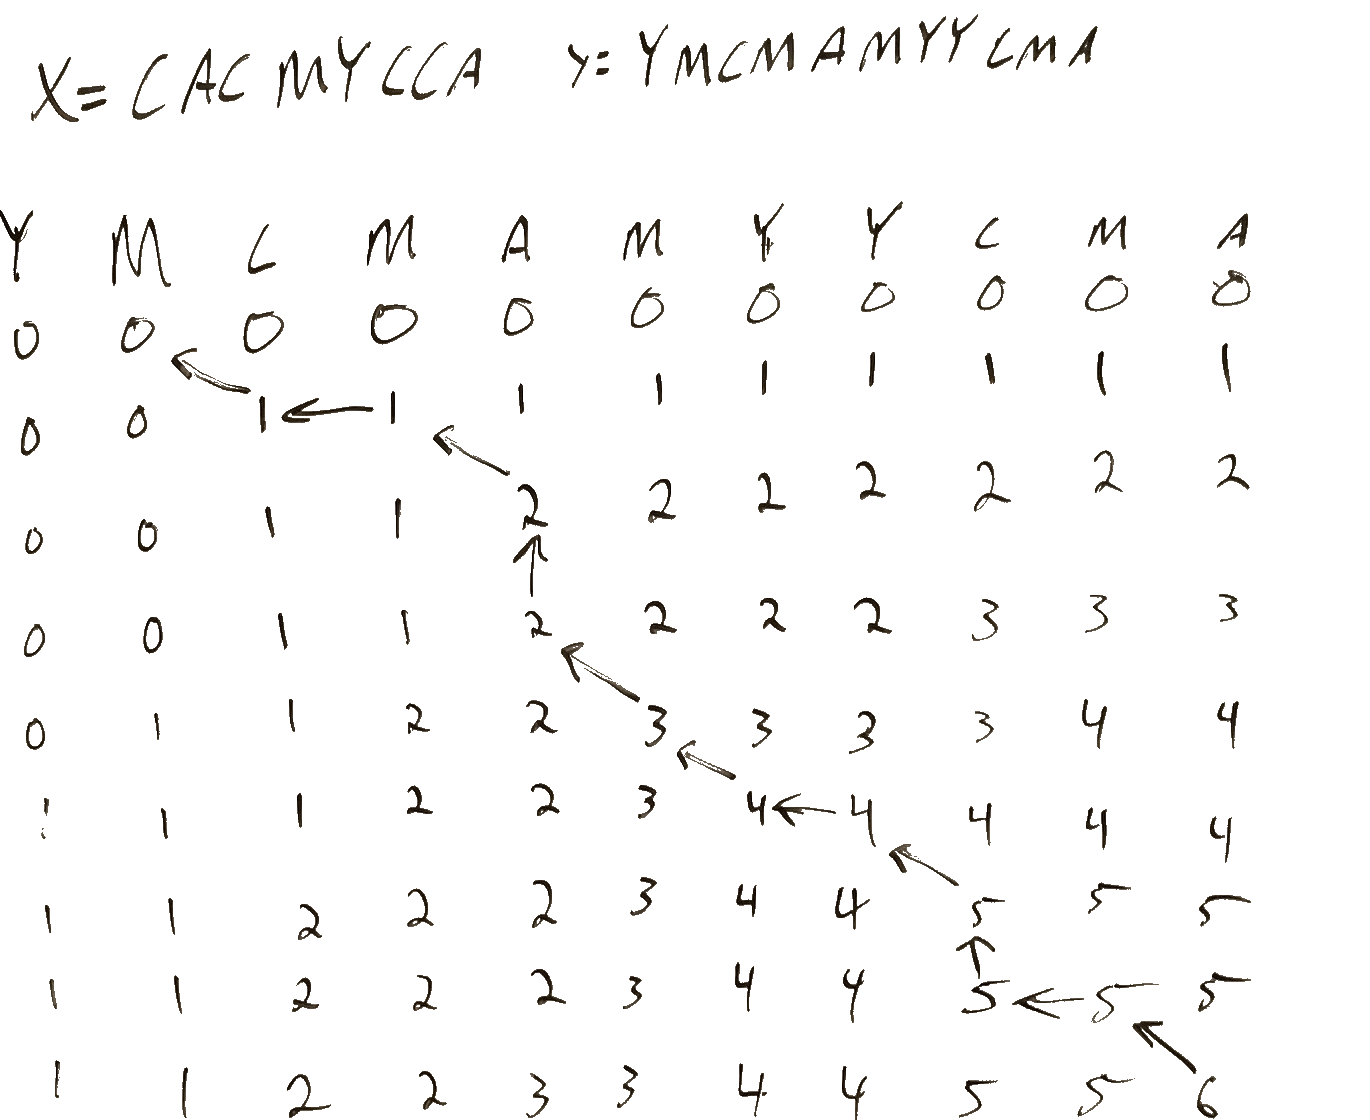
\includegraphics[width=15cm]{lcs}

\section{Floyd's Algorithm}
6 iterations.

$D^0, P^0$

\begin{tabular}{ | l | c | c | c | r | }
  \hline
  0 & 2 & - & 1 & 8 \\ \hline
  6 & 0 & 3 & 2 & - \\ \hline
  - & - & 0 & 4 & - \\ \hline
  - & - & 2 & 0 & 3 \\ \hline
  3 & - & - & - & 0 \\ \hline
\end{tabular}
\quad
\begin{tabular}{ | l | c | c | c | r | }
  \hline
  - & 2 & - & 4 & 5 \\ \hline
  1 & - & 3 & 4 & - \\ \hline
  - & - & - & 4 & - \\ \hline
  - & - & 3 & - & 5 \\ \hline
  1 & - & - & - & - \\ \hline
\end{tabular}

$D^1, P^1$

\begin{tabular}{ | l | c | c | c | r | }
  \hline
  0 & 2 & - & 1 & 8 \\ \hline
  6 & 0 & 3 & 2 & 14 \\ \hline
  - & - & 0 & 4 & - \\ \hline
  - & - & 2 & 0 & 3 \\ \hline
  3 & 5 & - & 4 & 0 \\ \hline
\end{tabular}
\quad
\begin{tabular}{ | l | c | c | c | r | }
  \hline
  - & 2 & - & 4 & 5 \\ \hline
  1 & - & 3 & 4 & 1 \\ \hline
  - & - & - & 4 & - \\ \hline
  - & - & 3 & - & 5 \\ \hline
  1 & 1 & - & 1 & - \\ \hline
\end{tabular}

$D^2, P^2$

\begin{tabular}{ | l | c | c | c | r | }
  \hline
  0 & 2 & 5 & 1 & 8 \\ \hline
  6 & 0 & 3 & 2 & 14 \\ \hline
  - & - & 0 & 4 & - \\ \hline
  - & - & 2 & 0 & 3 \\ \hline
  3 & 5 & - & 4 & 0 \\ \hline
\end{tabular}
\quad
\begin{tabular}{ | l | c | c | c | r | }
  \hline
  - & 2 & 2 & 4 & 5 \\ \hline
  1 & - & 3 & 4 & 1 \\ \hline
  - & - & - & 4 & - \\ \hline
  - & - & 3 & - & 5 \\ \hline
  1 & 1 & - & 1 & - \\ \hline
\end{tabular}

$D^3, P^3$

\begin{tabular}{ | l | c | c | c | r | }
  \hline
  0 & 2 & 5 & 1 & 8 \\ \hline
  6 & 0 & 3 & 2 & 14 \\ \hline
  - & - & 0 & 4 & - \\ \hline
  - & - & 2 & 0 & 3 \\ \hline
  3 & 5 & - & 4 & 0 \\ \hline
\end{tabular}
\quad
\begin{tabular}{ | l | c | c | c | r | }
  \hline
  - & 2 & 2 & 4 & 5 \\ \hline
  1 & - & 3 & 4 & 1 \\ \hline
  - & - & - & 4 & - \\ \hline
  - & - & 3 & - & 5 \\ \hline
  1 & 1 & - & 1 & - \\ \hline
\end{tabular}

$D^4, P^4$

\begin{tabular}{ | l | c | c | c | r | }
  \hline
  0 & 2 & 3 & 1 & 4 \\ \hline
  6 & 0 & 3 & 2 & 5 \\ \hline
  - & - & 0 & 4 & 7 \\ \hline
  - & - & 2 & 0 & 3 \\ \hline
  3 & 5 & - & 4 & 0 \\ \hline
\end{tabular}
\quad
\begin{tabular}{ | l | c | c | c | r | }
  \hline
  - & 2 & 4 & 4 & 4 \\ \hline
  1 & - & 3 & 4 & 5 \\ \hline
  - & - & - & 4 & 4 \\ \hline
  - & - & 3 & - & 5 \\ \hline
  1 & 1 & - & 1 & - \\ \hline
\end{tabular}

$D^5, P^5$

\begin{tabular}{ | l | c | c | c | r | }
  \hline
  0 & 2 & 3 & 1 & 4 \\ \hline
  6 & 0 & 3 & 2 & 5 \\ \hline
  - & - & 0 & 4 & 7 \\ \hline
  6 & - & 2 & 0 & 3 \\ \hline
  3 & 5 & - & 4 & 0 \\ \hline
\end{tabular}
\quad
\begin{tabular}{ | l | c | c | c | r | }
  \hline
  - & 2 & 4 & 4 & 4 \\ \hline
  1 & - & 3 & 4 & 5 \\ \hline
  - & - & - & 4 & 4 \\ \hline
  5 & - & 3 & - & 5 \\ \hline
  1 & 1 & - & 1 & - \\ \hline
\end{tabular}

\section{Merge Heap}
The proposed algorithm is incorrect, sift down must be called on every node before n/2, where
n is the size of the entire heap. Since $n_2 \geq n_1$, the algorithm will only be correct when
$n_1 == n_2$.
\begin{lstlisting}
for (i = 1; i <= n2, i++):
    bt1[n1 + i] = bt2[i]
last = n1 + n2
for (i = last / 2; i > 0, i--):
    siftDown(bt1, i)
\end{lstlisting}
This algorithm will run in $\Theta(n_2) + \Theta(n_1 + n_2)$

\section{Binomial Coefficient}

$\binom{8}{6} = 28$
\vspace{0.5em}

\begin{tabular}{ | l || c | c | c | c | c | c | c | c | r | }
  \hline
    & 0 & 1 & 2 & 3 & 4 & 5 & 6 & 7 & 8\\ \hline\hline
  0 & 1 \\ \hline
  1 & 1 & 1  \\ \hline
  2 & 1 & 2 & 1 \\ \hline
  3 & 1 & 3 & 3 & 1 \\ \hline
  4 & 1 & 4 & 6 & 4 & 1 \\ \hline
  5 & 1 & 5 & 10 & 10 & 5 & 1\\ \hline
  6 & 1 & 6 & 15 & 20 & 15 & 6 & 1\\ \hline
  7 & 1 & 7 & 21 & 35 & 35 & 21 & 7 & 1\\ \hline
  8 & 1 & 8 & 28 & 56 & 70 & 56 & 28 & 8 & 1\\ \hline
\end{tabular}

\vspace{1em}
Compute $\binom{8}{8-6}$ instead
\vspace{0.5em}

\begin{tabular}{ | l || c | c | c |}
  \hline
     & 0 & 1 & 2 \\ \hline\hline
  0  & 1 \\ \hline
  1  & 1 & 1 \\ \hline
  2  & 1 & 2 & 1 \\ \hline
  3  & 1 & 3 & 3 \\ \hline
  4  & 1 & 4 & 6 \\ \hline
  5  & 1 & 5 & 10 \\ \hline
  6  & 1 & 6 & 15 \\ \hline
  7  & 1 & 7 & 21 \\ \hline
  8  & 1 & 8 & 28 \\ \hline
\end{tabular}

\section{Sum of Subsets}
\subsection{Recurrence}
$$A_{i,s} = A_{i, s-1}\ ||\ A_{i - p[s], s-1$$

\subsection{Pseudo Code}
\begin{lstlisting}
  for i in B:
    for j in B[i]:
      if p[i] >= y:
        B[i][j] = B[i-1][j]
      else:
        B[i][j] = B[i-1][j-p[i]]
\end{lstlisting}

\subsection{Example}
\begin{tabular}{ | l || c | c | c | c | c | c | c |}
  \hline
    & 0 & 1 & 2 & 3 & 4 & 5 & 6 \\ \hline\hline
  1 & \uparrow T & T & F & F & F & F & F\\ \hline
  2 & \uparrow T & \uparrow T & T & T & F & F & F\\ \hline
  4 & \uparrow T & \uparrow T & \uparrow T & \uparrow T & T & T & T\\ \hline
\end{tabular}


\end{document}
